\documentclass[a4paper, french, 12pt]{report}
\usepackage[utf8]{inputenc}
\usepackage[T1]{fontenc}
\usepackage[french]{babel}

\usepackage{nccmath}
\usepackage{amsmath}
\usepackage{amssymb}
\usepackage{graphicx}
\usepackage{caption}
\usepackage{eso-pic}

\usepackage[margin=2cm, bottom=1.5cm, includefoot, footskip=30pt]{geometry}
\usepackage[pdftex, pdfauthor={Anas HAFSI}, pdftitle={Rapport de stage de fin d'études}, pdfsubject={Rapport PFE Anas HAFSI}, pdfkeywords={Java, Angular, Amundi, Finaxys}, pdfborder={0 0 0}]{hyperref}

\usepackage{enumitem}
\setlist[enumerate]{after={\bigskip}}
\setlist[itemize]{after={\bigskip}}

\usepackage{lastpage}
\usepackage{fancyhdr}
\usepackage{subfig}
\pagestyle{fancy}

\usepackage{pdfpages}
\usepackage{perpage}
\MakePerPage{footnote}
\usepackage{tabto}
\usepackage{tabularx}

\AddThinSpaceBeforeFootnotes
\FrenchFootnotes

\usepackage{appendix}
\usepackage{listings}


% VARIABLES

\makeatletter
\title{Rapport du projet de fin d'études}\let\title\@title
\newcommand{\subtitle}{Master Data Management - Media Plus Core}
\newcommand{\years}{2019 - 2020}
\newcommand{\footpage}{ Page \thepage \ / \pageref{LastPage}}

% CONFIG 


\@addtoreset{chapter}{part}
\renewcommand{\headrulewidth}{0pt}
\renewcommand{\footrulewidth}{0pt}

\newcommand{\HRule}{\rule{\linewidth}{0.5mm}}
\newcommand{\blap}[1]{\vbox to 0pt{#1\vss}}
\newcommand\AtUpperLeftCorner[3]{%
  \put(\LenToUnit{#1},\LenToUnit{\dimexpr\paperheight-#2}){\blap{#3}}%
}
\newcommand\AtUpperRightCorner[3]{%
  \put(\LenToUnit{\dimexpr\paperwidth-#1},\LenToUnit{\dimexpr\paperheight-#2}){\blap{\llap{#3}}}%
}

\renewcommand{\chaptername}{Chapitre}



\begin{document}

\begin{titlepage}
  \begin{titlepage}
	\enlargethispage{2cm}

	\AddToShipoutPicture{
		\AtUpperLeftCorner{2cm}{1.5cm}{
\includegraphics[width=6cm]{img/logo_ecole.jpg}}
		\AtUpperRightCorner{2cm}{2cm}{
\includegraphics[width=5cm]{img/logo_univ.png}}
	}
	
	\vspace*{8cm}

	\begin{center}
		\vbox{\underline{\LARGE{\title}} : }
		\vspace*{0.5cm}
		\vbox{\LARGE{\subtitle}}
		\vspace*{0.5cm}
		\HRule
		\vspace*{0.5cm}
	\end{center}

	\begin{center}
		\mbox{\textbf{Etablissement : } Ecole nationale des sciences appliquées d'Oujda}\\
		\mbox{\textbf{Etablissement d'acceuil: } Ecole d'ingénieurs Sup Galilée}\\
		\mbox{\textbf{Spécialité : } Informatique}\\
		\mbox{\textbf{Année scolaire : } Troisième année - équivalent M2}\\
		\mbox{\textbf{Lieu : } Université Sorbonne Paris Nord - 93430 Villetaneuse}
	\end{center}
	\begin{center}
		\mbox{\textbf{Soutenu par:} Anas HAFSI}\\
	\end{center}

	\vspace*{6.8cm}

	\begin{flushright} \large
		\emph{Année universitaire : \years}\\
	\end{flushright}

\end{titlepage}
\end{titlepage}


\ClearShipoutPicture
\newpage


% ----------------------------------------------------------------------------------------
%                                 Report essential Sections
% ----------------------------------------------------------------------------------------

\newenvironment{dedication}
     {\vspace{6ex}\begin{quotation}\begin{center}\begin{em}}
     {\par\end{em}\end{center}\end{quotation}}

     \begin{dedication}
A mes parents, ma famille, mes amis et a la rue Guynemer squad.
\end{dedication}
\newpage
\newenvironment{remerciment}
     {\vspace{6ex}\begin{quotation}\begin{center}\begin{em}}
     {\par\end{em}\end{center}\end{quotation}}

     \begin{remerciment}
\par I'd like to thank myself \\
\par To love mankind FOR GOD'S SAKE—this has so far been the noblest and remotest sentiment to which mankind has attained. That love to mankind, without any redeeming intention in the background, is only an ADDITIONAL folly and brutishness, that the inclination to this love has first to get its proportion, its delicacy, its gram of salt and sprinkling of ambergris from a higher inclination—whoever first perceived and "experienced" this, however his tongue may have stammered as it attempted to express such a delicate matter, let him for all time be holy and respected, as the man who has so far flown highest and gone astray in the finest fashion!   
     \end{remerciment}
\chapter*{Résumé}
\par Le présent rapport synthétise le travail effectué au sein de l'entreprise Finaxys et son client Amundi AM, dans le cadre du stage pour l’obtention du diplôme Ingénieur d'état Spécialité : Génie des Systèmes Électroniques Informatiques et Réseaux de l'École Nationale des Sciences Appliquées d'Oujda.  \\
\par Parmis les nombreux clients de Finaxys, société de consultants spécialisée en IT finance, Amundi AM est considéré comme un client stratégique. Le leader européen et mondial qui opère dans le domaine de la gestion d'actifs, est subdivisé en plusieurs sous entités. J'ai été assignée au service OST/ITS/INV/MDM, MDM pour Master Data Management. \\
\par MDM regroupe toutes les équipes gérant des applications qui utilisent des données sensible d'Amundi AM nommée Master Data. J'ai ete assignée a deux projets majeurs, Media Plus Core et Alto Investment Research. \\
\par MediaplusCore est une application/Serveur chargé de diffuser plusieurs données marché a ses utilisateurs. On retrouve par exemple des données portefeuille, des données indices, etc\dots Le serveur est développé sous JAVA 7 puis on a réalisé une migration vers JAVA 8 vers septembre 2020. J'ai eu la chance d'interagir avec plusieurs parties du projet, pour mon stage de fin d'études, notamment la creations de nouveaux API REST et l'ajout et modification d'EJB. \\
\par Alto Investment Research est une application front office développé avec Maestro, un framework basé sur le framework Angular 8, dont le but est de fournir et transformer une ancienne interface vers de nouveaux écrans crée par des designers UI/UX afin d'offrir au utilisateurs une interface complete et facile d'utilisation. Cette Application est notamment utilisé par les ingénieurs métiers Amundi AM (Traders, Commerciaux\dots). \\
\par Des outils de gestion comme Jira et Gitlab sont utilisés quotidiennement par les membres de l’équipe développant les deux projets.
\\~\\~\\~\\~\\~\\~\\~\\
\par Mots clés: JAVA, Angular, Maestro, Jira, Gitlab, Asset Management, Amundi, Finaxys

\chapter*{Abstract}
    This is the abstract document


% ----------------------------------------------------------------------------------------
%                                 Tables of Content/tables/figures/abrv
% ----------------------------------------------------------------------------------------

\tableofcontents
\listoftables
\listoffigures
\chapter*{Liste des abréviations, sigles et acronymes}
\par \textbf{AM}: Asset Management \\
\par \textbf{Alto}: Amundi Leading Technologies and Operations \\
\par \textbf{Amundi AM}: Amundi Asset Management \\
\par \textbf{BFTIM}: BFT Investment Managers \\
\par \textbf{BFI}: Banque de Financement et d'Investissement \\
\par \textbf{CAAM}: Crédit agricole Asset Management \\
\par \textbf{CASAM}: Crédit agricole Structured Asset Management \\
\par \textbf{CEA}: Commissariat à l'énergie atomique et aux énergies alternatives\\
\par \textbf{Critères ESG}: Critères environnementaux et sociaux de gouvernance\\
\par \textbf{CPR}: Compagnie parisienne de réescompte \\
\par \textbf{ETF}: Exchange Traded Fund : Fonds négocié en bourse\\
\par \textbf{FCP}: Fonds commun de placement \\
\par \textbf{GmbH}: Gesellschaft mit beschränkter Haftung \\
\par \textbf{Inc}: Incorporation \\
\par \textbf{ISR}: Investissement socialement responsable \\
\par \textbf{LCL}: Le Crédit lyonnais \\
\par \textbf{LLC}: Limited liability company \\
\par \textbf{MIF}: Marchés d'instruments financiers \\
\par \textbf{MIFID}: Markets in Financial Instruments Directive \\
\par \textbf{OPCVM}: Organisme de placement collectif en valeurs mobilières \\
\par \textbf{SGAM}: Société générale Asset Management \\
\par \textbf{SGIIC}: Sociedad Gestora de Instituciones de Inversión Colectiva \\
\par \textbf{SGR}: Societa Di Gestione Del Risparmio \\
\par \textbf{SICAV}: Société d'investissement à capital variable \\
\par \textbf{SOLID}: Single responsibility, Open/close, Liskov Substitution, Interface segregation, Dependency inversion \\
\par \textbf{S.A.}: Société anonyme \\
\par \textbf{VEFA}: Vente en l'état futur d'achèvement \\
\par \textbf{VL}: Valeur Liquidative \\
\par \textbf{xDD}: x Driven Design \\
\clearpage

% ----------------------------------------------------------------------------------------
%                                 Head/Foot Configuration
% ----------------------------------------------------------------------------------------

\fancyhead{}
\fancyhead[RO,LE]{Rapport PFE}
\fancyfoot{}
\fancyfoot[LE,RO]{\thepage}
\fancyfoot[LO,CE]{Partie \thepart\ Chapitre \thechapter}
% \fancyfoot[CO,RE]{Anas HAFSI}

% ----------------------------------------------------------------------------------------
%                                 Parts/Chapters
% ----------------------------------------------------------------------------------------
\chapter*{Introduction}
Riche d’expérience professionnelle divers (Projets, stages\dots), je n’avais  toutefois jamais eu l’opportunité d’une véritable expérience sur une longue  durée, en tant que jeune ingénieur avant ce stage, d’où l’importance capitale  de celle-ci. \\
\par Mon stage porte sur l’intégration dans un premier temps chez Finaxys  Academy, une université interne incubatrice des jeunes talents, pour intégrer  par la suite le département OST/ITS/INV/MDM d'Amundi Asset Management chargé de fournir plusieurs informations critiques, nommée Master Data: des Equity, des Issuers, des Portfolios\dots . Ces différentes activités  s’inscrivent également dans le respect des régulations de plus en plus forte sur  les marchés financiers. \\
\par C’est dans ce sillage que j’ai rejoint pour le compte de Finaxys, Amundi Asset Management, en tant qu’ingénieur  d’études et développement sur le projet MediaPlus-Core \& Alto (Amundi Leading Technology and Operations) Investment Research, Deux projets central dans l'écosystème Amundi AM. \\
\par Ma mission au sein de l’équipe m’a amené à participer à l’étude et l’analyse  du besoin, au développement d'Ejb, des web services et également à la creation de widgets, de vues et d'interfaces graphiques.
\addcontentsline{toc}{part}{Introduction}
\part{Contexte général du projet}
% Chapter Template

\chapter{Organisme d’accueil} % Main chapter title

\label{Chapter01} % Change X to a consecutive number; for referencing this chapter elsewhere, use \ref{ChapterX}

\par
Avant d'entamer l’analyse du projet il est essentiel de commencer par une présentation générale des entités d’accueil, ceci en introduisant l'historique ainsi que les produits. Et donc par conséquent, Ce chapitre est une présentation sommaire du contexte de notre projet de fin d’études. Il comporte deux grandes parties : dans la première, nous allons présenter l’entreprise d’accueil Finaxys, puis nous allons présenter Amundi Asset Manager, le client de Finaxys chez lequel j'ai pu réaliser le projet.
Chaque partie est subdivisée en plusieurs sous-partie : nous exposeront l'historique de chaque entreprise, nous allons dévoiler les chiffres clés démontrant son succès économique. Nous allons ensuite expliquer brièvement l'organisation fonctionnelle ainsi que les différentes équipes de IT avec lequelle j'ai eu la chance d'interagir XX ainsi que sa démarche qualité pour la gestion de ses projets. Dans la seconde partie, nous présenterons notre client et développerons le cadre général du projet CDL; Carnet de Liaison en présentant brièvement ses modules, notamment les modules Adhérent et Suivi qui font l’objet de notre PFE. Dans la dernière partie, nous allons révéler la conduite de projet pour laquelle nous avons opté afin de mener efficacement notre projet.XX


\section{Finaxys}
\par
Finaxys est une société de consultants spécialisée en IT finance, banque et assurance. Elle permet aux acteurs de ce marché de bénéficier d’experts pour l’analyse, le cadrage et la définition des projets IT, comme pour leur déploiement et implémentation.
\subsection{Historique}

Nunc posuere quam at lectus tristique eu ultrices augue venenatis. Vestibulum ante ipsum primis in faucibus orci luctus et ultrices posuere cubilia Curae; Aliquam erat volutpat. Vivamus sodales tortor eget quam adipiscing in vulputate ante ullamcorper. Sed eros ante, lacinia et sollicitudin et, aliquam sit amet augue. In hac habitasse platea dictumst.

%-----------------------------------
%	SUBSECTION 2
%-----------------------------------

\subsection{Domaine d'activité}
Morbi rutrum odio eget arcu adipiscing sodales. Aenean et purus a est pulvinar pellentesque. Cras in elit neque, quis varius elit. Phasellus fringilla, nibh eu tempus venenatis, dolor elit posuere quam, quis adipiscing urna leo nec orci. Sed nec nulla auctor odio aliquet consequat. Ut nec nulla in ante ullamcorper aliquam at sed dolor. Phasellus fermentum magna in augue gravida cursus. Cras sed pretium lorem. Pellentesque eget ornare odio. Proin accumsan, massa viverra cursus pharetra, ipsum nisi lobortis velit, a malesuada dolor lorem eu neque.gfd

\subsection{Fiche Technique}

\def\arraystretch{1.8}
\begin{center}
    \begin{tabularx}{0.8\textwidth} { 
        | >{\raggedright\arraybackslash}X
        | >{\centering\arraybackslash}X | }
    \hline
    Nom de la société   &   Finaxys \\
    \hline
    Statut Juridique    &   Société par actions simplifiée (SAS) \\
    \hline
    Siege social        &   Tour INITIALE – 1 Terrasse Bellini,  92919 Paris la Défense  \\
    \hline
    Nombre de sites     &   3 (Paris, Londres, Bruxelles) \\
    \hline
    Date de création    &   Novembre 2003  \\
    \hline
    Secteur d’activité  &   Conseil en systèmes et logiciels informatiques  \\
    \hline
    Chiffre d’affaire   &   + 41.7 Millions d'Euros (2018)  \\
    \hline
    Clients principaux  &   Amundi Asset Management, Société Générale, BNP Paribas, HSBC \dots  \\
    \hline
    Effectif            &   230 employés\\
    \hline
    Certification       &   XXXXXXXXX  \\
    \hline
    \end{tabularx}
    \begin{table}[htp]
        \caption{Fiche Technique Finaxys}
    \end{table}
\end{center}

\section{Amundi Asset Management}

Sed ullamcorper quam eu nisl interdum at interdum enim egestas. Aliquam placerat justo sed lectus lobortis ut porta nisl porttitor. Vestibulum mi dolor, lacinia molestie gravida at, tempus vitae ligula. Donec eget quam sapien, in viverra eros. Donec pellentesque justo a massa fringilla non vestibulum metus vestibulum. Vestibulum in orci quis felis tempor lacinia. Vivamus ornare ultrices facilisis. Ut hendrerit volutpat vulputate. Morbi condimentum venenatis augue, id porta ipsum vulputate in. Curabitur luctus tempus justo. Vestibulum risus lectus, adipiscing nec condimentum quis, condimentum nec nisl. Aliquam dictum sagittis velit sed iaculis. Morbi tristique augue sit amet nulla pulvinar id facilisis ligula mollis. Nam elit libero, tincidunt ut aliquam at, molestie in quam. Aenean rhoncus vehicula hendrerit.
\subsection{Un Asset Manager}

\par Par abus de langage le terme « asset manager » est ici utilisé pour décrire le marché des biens immobiliers ; les Anglo-saxons associent le terme asset management à une gestion beaucoup plus étendue d'actifs, comprenant entre autres les obligations, les actions, les produits dérivés, les matières premières...
\par L’asset manager immobilier est un terme anglo-saxon, apparu en France dans les années 1990, qui définit le métier de gestionnaire d'actifs immobiliers d'entreprise comme un ensemble de services aux propriétaires, de l'acquisition du bien à sa cession.
\par L’asset manager immobilier est le responsable de la gestion d'un portefeuille d'actifs immobiliers pour le compte de tiers.
\par Il est le garant de la rentabilité des biens immobiliers attendue par les investisseurs, assurée par sa connaissance polyvalente des marchés de l'immobilier d'entreprise et d'habitation, sa maîtrise des baux commerciaux et du droit immobilier, ses compétences financières tant au plan de la modélisation de flux de trésorerie et scénarios immobiliers qu'il doit optimiser que du reporting aux investisseurs, sa capacité à penser et suivre des plans de travaux sur les immeubles, de la restructuration lourde au développement et son talent de négociateur tant pour la commercialisation des actifs que pour ses relations avec les différents intervenants et prestataires extérieurs.
\par Ce métier est apparu en France vers la fin des années 1990, après la crise immobilière sans précédent qu'avait connue le pays, à la suite de la spéculation de nombreux acteurs financiers anglo-saxons qui avaient su saisir les opportunités durant cette période et avaient en particulier apporté des techniques d'investissement et de gestion encore inconnues en France.
\par Une pyramide des métiers s'est créée et régit aujourd'hui le secteur de l'immobilier d'entreprise : l’investment manager immobilier (responsable d'investissements), l’asset manager immobilier (gestionnaire d'actifs immobilier représentant du propriétaire), le fund manager immobilier (responsable de fonds d'investissement immobilier), le portfolio manager immobilier (responsable des relations avec les clients et du reporting financier), le property manager (gestionnaire locatif et technique), le facility manager (responsable des services aux utilisateurs de l'immeuble).
\par Selon les sociétés, il est possible de trouver des définitions différentes de ces métiers ; l’asset manager immobilier peut ainsi, en sus de sa casquette de gestionnaire, être responsable de l'investissement en amont et de la vente de l'actif à un tiers.
\par L’asset manager immobilier exerce son métier sur des types d'actifs variés : bureaux, centres commerciaux, commerces de pied d'immeuble, logistique, entrepôts, habitation, hôtels… Il se doit de maîtriser les particularités afférentes à chacun de ces secteurs d'activités, par exemple : le marché de l'emploi et du tertiaire pour les bureaux, l'actualité des enseignes et la consommation des ménages pour le commerce, la réglementation des installations classées pour la logistique, etc.

\subsection{Historique}

Nunc posuere quam at lectus tristique eu ultrices augue venenatis. Vestibulum ante ipsum primis in faucibus orci luctus et ultrices posuere cubilia Curae; Aliquam erat volutpat. Vivamus sodales tortor eget quam adipiscing in vulputate ante ullamcorper. Sed eros ante, lacinia et sollicitudin et, aliquam sit amet augue. In hac habitasse platea dictumst.

%-----------------------------------
%	SUBSECTION 2
%-----------------------------------

\subsection{Domaine d'activité}
Morbi rutrum odio eget arcu adipiscing sodales. Aenean et purus a est pulvinar pellentesque. Cras in elit neque, quis varius elit. Phasellus fringilla, nibh eu tempus venenatis, dolor elit posuere quam, quis adipiscing urna leo nec orci. Sed nec nulla auctor odio aliquet consequat. Ut nec nulla in ante ullamcorper aliquam at sed dolor. Phasellus fermentum magna in augue gravida cursus. Cras sed pretium lorem. Pellentesque eget ornare odio. Proin accumsan, massa viverra cursus pharetra, ipsum nisi lobortis velit, a malesuada dolor lorem eu neque.



\subsection{Fiche Technique}

\begin{center}
    \begin{tabularx}{0.8\textwidth} { 
        | >{\raggedright\arraybackslash}X
        | >{\centering\arraybackslash}X | }
    \hline
    Nom de la société   &   Amundi Asset Management - Amundi AM \\
    \hline
    Statut Juridique    &   Société par actions simplifiée (SAS)  \\
    \hline
    Siege social        &   90, boulevard Pasteur - 75015 Paris  \\
    \hline
    Siege social        &   + 40 Pays (Dont Tokyo, Dublin, Boston, Londres \dots) \\
    \hline
    Date de création    &   Avril 2001  \\
    \hline
    Secteur d’activité  &   Gestion de fonds  \\
    \hline
    Chiffre d’affaire   &   + 1,17 Milliard d'Euros (2018)  \\
    \hline
    Fonds sous gestion  &   + 1600 Milliard d'Euros (2019)  \\
    \hline
    Clients             &   + 100 Millions (dont 1500 clients institutionnels)  \\
    \hline
    Effectif            &   2000 employés\\
    \hline
    Certification       &   XXXXXXXXX  \\
    \hline
    \end{tabularx}
    \begin{table}[htp]
        \caption{Fiche Technique Amundi AM}
    \end{table}
\end{center}
\part{Étude technico-fonctionnelle}
Une étape cruciale dans le cycle de développement des systèmes software adopté par toute société respectant
les normes et standards du domaine automobile est l’ingénierie des exigences (RE). Celle-ci fut créée comme
sous-domaine de l’ingénierie logicielle avec la tâche de développer des modèles, des techniques et des outils qui
permettent de hiérarchiser les exigences d’un projet, de détecter les incohérences entre elles et d’assurer leur
traçabilité. Elle permet donc d’éviter des frais onéreux engendrés par une maintenance couteuse des systèmes
logiciels, due à des erreurs au niveau de la définition des exigences, qui pourrait même entrainer à un rejet total,
au pire des cas.
L’ingénierie des exigences s’articule principalement sur deux phases : la définition des exigences (RD) et la
gestion des exigences (RM). Le développement des exigences permet d’obtenir un ensemble de spécifications
convenues. Cependant, les changements de ces spécifications sont souvent inéluctables, et les facteurs sont multiples : nouvelles priorités d’affaires, découverte de nouvelles exigences, etc. La gestion des exigence, quant à
elle, surveille les changements et garantit que les exigences sont modifiées de manière contrôlée, en maintenant
la traçabilité tout au long de la réalisation du projet.
C’est dans ce cadre que Lear CORPORATION a adopté l’outil Rational Doors, et a développé l’outil ReqTool, qui exploite les données de DOORS ainsi que différentes sources additionnelles (SQA, ReqDB ...) pour
générer des rapports et des matrices de traçabilités. Néanmoins, ces derniers restent peu pratiques due à leur
format apathique et non intuitif. De plus, bien qu’il soit nécessaire de les générer plusieurs fois par jour, le
temps de génération est si important qu’on ne peut se permettre de le faire que deux à trois fois au plus, par
jour. Une révision de l’outil s’impose donc, afin de l’optimiser.
Mots-clés : Gestion des exigences, Cycle en V, Rational DOORS, DXL, ReqTool, Modélisation des données,
Spring Boot, ReactJs, JEE, Micro-services.
\pagebreak
\part{Étude technique et réalisations}
\par Dans la présente Section, on va découvrir ce qui a été concrètement réaliser durant le stage, ainsi que tout les outils utilisés pour mener a bien les différents projets. J'essayerais, par la suite, de présenter un bilan général des six mois de stage.  

\begingroup
    \let\clearpage\relax
    \chapter{Environnement technique et outils technologiques}
\endgroup
\section{Outils communs}
\par Dans la présente section, je présenterais tout les outils commun a tout les projets, notamment les outils fonctionnels (outils de planification \dots) ainsi que les outils pour vérifier la qualité du code et déploiement des applications. 
\subsection{La suite Atlassian}
\par Atlassian est un éditeur de logiciels, basé en Australie, qui développe des produits pour la gestion de développement et de projets. Ses logiciels les plus connus sont Jira, Confluence, Bamboo, Bitbucket et Trello. Une grande parte de la suite Atlassian est payante.
\par Pour nos projets, j'ai pu utiliser JIRA et Confluence.

\subsubsection{Jira}
\par JIRA est un « issue tracker ». On pourrait traduire : un « Gestionnaire de demande ». Cette définition donne une idée du potentiel de l’outil mais reste néanmoins imparfaite parce que le terme anglais « Issue » fait référence à quelque chose de beaucoup plus générique. Une « Issue » est en fait un objet, sujet, ou situation, susceptible d’être traité. Il peut donc s’agir de bug, d’anomalies, d’incidents, de demandes d’intervention, mais aussi de la multitude des taches anodines qui font le quotidien de chacun d’entre nous. JIRA est un outil de suivi d’activités.
\clearpage
\par En pratique les cas d’utilisation de JIRA les plus souvent rencontrés sont les suivants :
\begin{itemize}
    \item La gestion du support et des activités de développement logiciel
    \item Le suivi des anomalies
    \item Le suivi d’activité
    \item La gestion de Centres de services
\end{itemize}
\begin{figure}[ht]
    \centering
    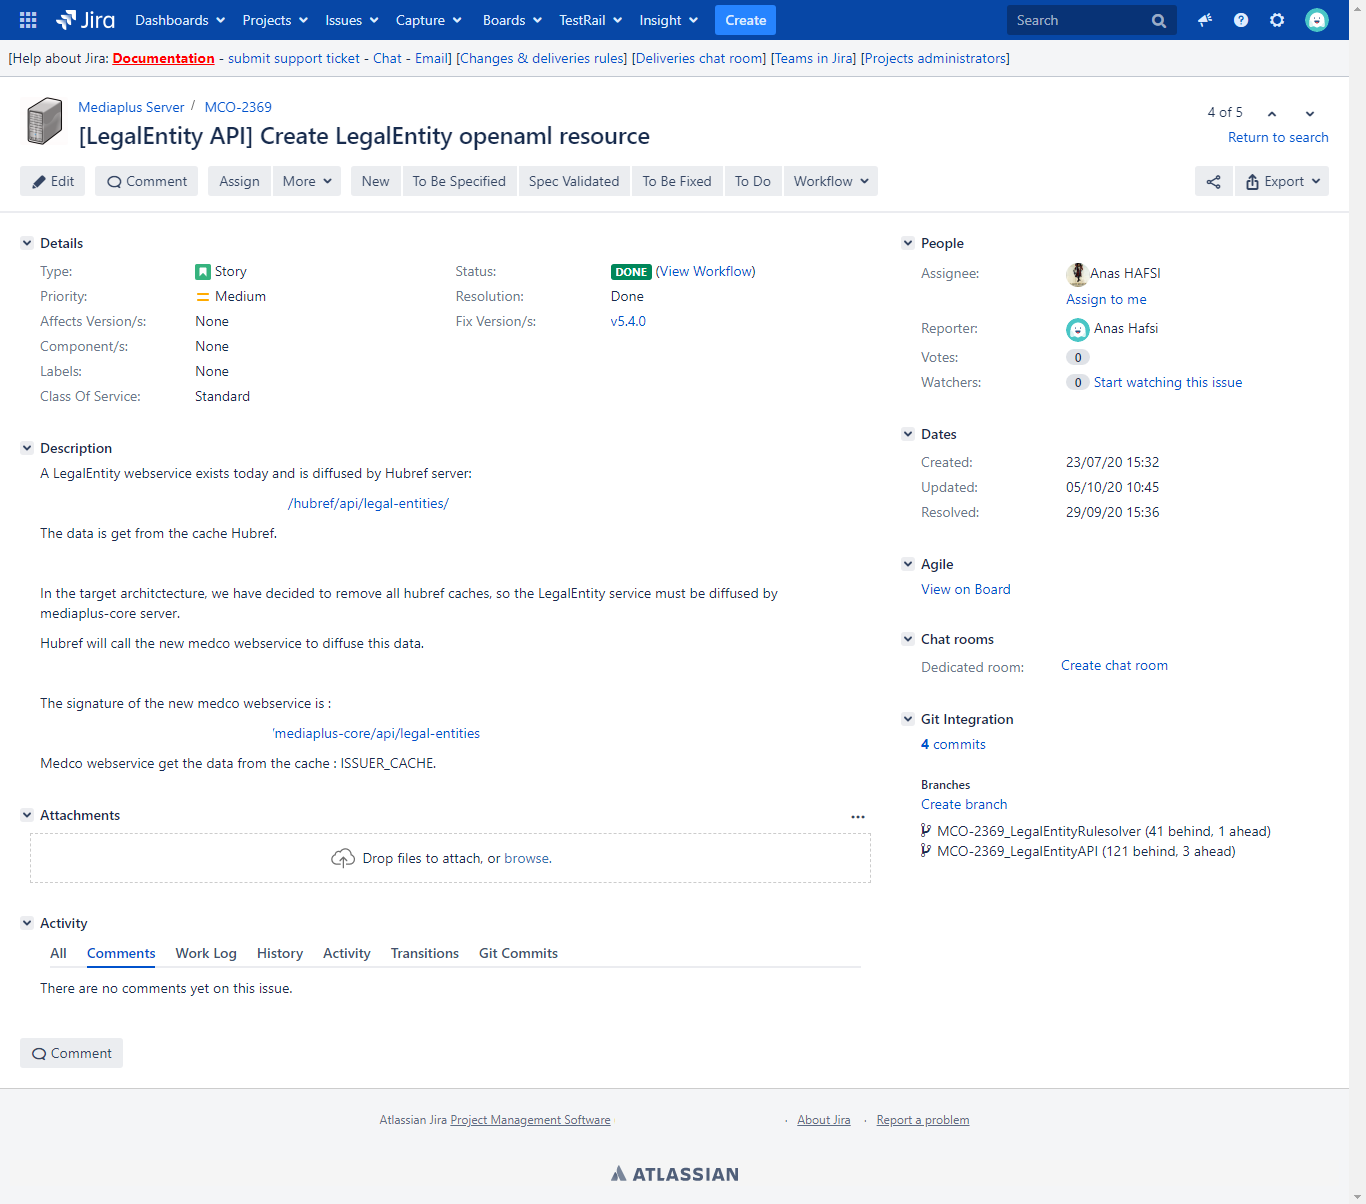
\includegraphics[width=\columnwidth]{img/JIRA MCO-2369.png}
    \caption{Ticket Jira MediaPlus Core}
    \label{fig:JiraMedco}
\end{figure}

\par Les "Issue" Jira sont nommée des tickets (exemple figure \ref{fig:JiraMedco}). l'ensemble de tickets appartenant au même sprint Agile sont rassemblé dans un "board JIRA" (exemple figure \ref{fig:JiraAlto}).
\clearpage
\begin{figure}[ht]
    \centering
    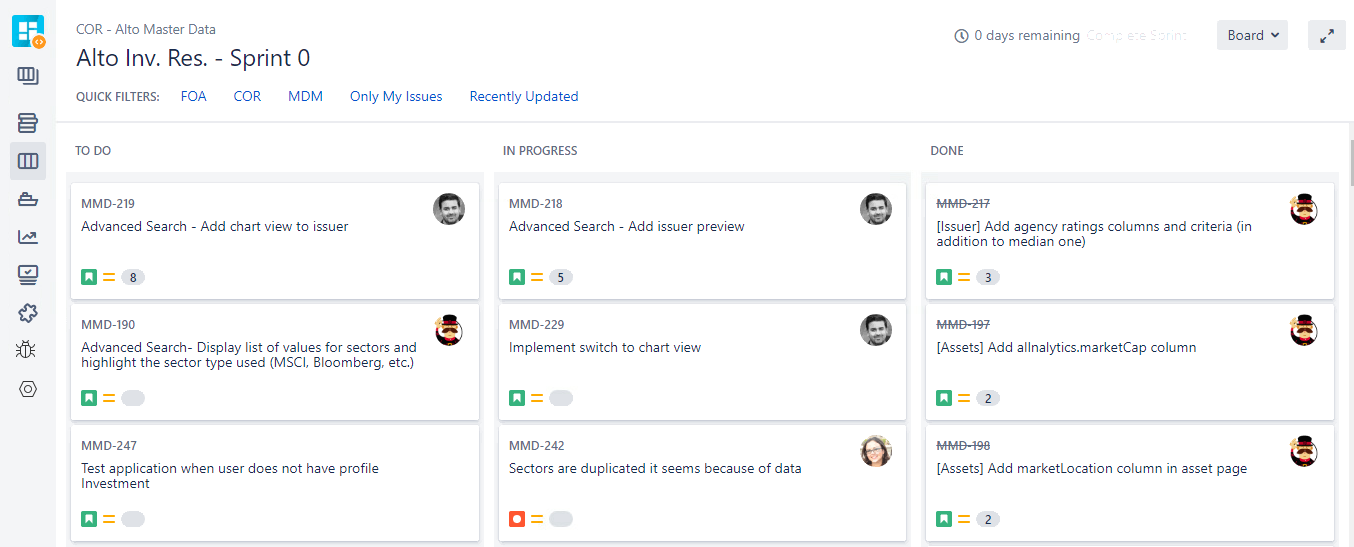
\includegraphics[width=\columnwidth]{img/Sprint Alto.png}
    \caption{Jira Board pour un sprint Alto Investment Research}
    \label{fig:JiraAlto}
\end{figure}
\subsubsection{Confluence}
\par Créez, collaborez et organisez tout votre travail à un seul et même endroit. Confluence est un espace de travail en équipe où la connaissance et la collaboration se rejoignent. Les pages dynamiques permettent à votre équipe de disposer d'un endroit pour créer, capturer et collaborer sur le projet ou l'idée de votre choix. Grâce aux espaces, votre équipe peut structurer, organiser et partager les tâches, afin que chacun de ses membres dispose d'une visibilité sur les connaissances institutionnelles ainsi que d'un accès aux informations nécessaires pour optimiser le travail.
\par Confluence s'adresse aux équipes de toute taille et de tout type. Qu'il s'agisse d'équipes ayant des projets stratégiques aux enjeux élevés, qui nécessitent de la rigueur dans leurs pratiques, ou d'équipes à la recherche d'un espace pour développer une culture d'équipe et interagir les unes avec les autres de manière plus ouverte et plus authentique. Grâce à Confluence, votre équipe peut prendre des décisions rapides, gagner en alignement et accomplir plus ensemble. {\tiny source: Atlassian documentation}
\par La figure \ref{fig:conf} représente un espace confluence.
\begin{figure}[ht]
    \centering
    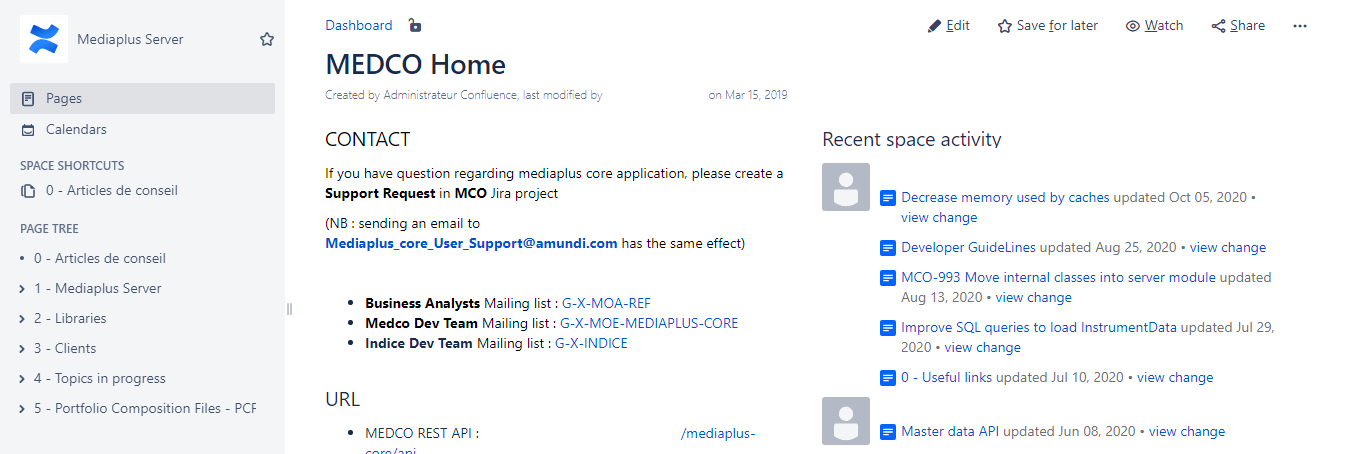
\includegraphics[width=\columnwidth]{img/ConfMedco.png}
    \caption{Espace Confluence MediaPlus-Core}
    \label{fig:conf}
\end{figure}

\subsection{Gitlab} 
\par GitLab est une plateforme de développement collaborative qui couvre l’ensemble des étapes du DevOps. Se basant sur les fonctionnalités du logiciel Git, elle permet de réaliser des dépôts et de gérer les versions de vos codes sources. Son usage est particulièrement indiqué pour les développeurs qui souhaitent disposer d’un outil réactif et accessible.
\par Comparé au autres logiciels de gestion de version, GitLab propose des options pour le moins pratiques :
\begin{itemize}
    \item Test de logiciels
    \item Configuration
    \item Monitoring
    \item Sécurité applicative
    \item Intégration et déploiement continus, etc\dots
\end{itemize}
\par Pour accompagner Gitlab on utilise SourceTree, un logiciel propriétaire du groupe Atlassian. C'est un logiciel front permettant de plus visualiser les branches git : un client frontend pour GitLab.
\begin{figure}[ht]
    \centering
    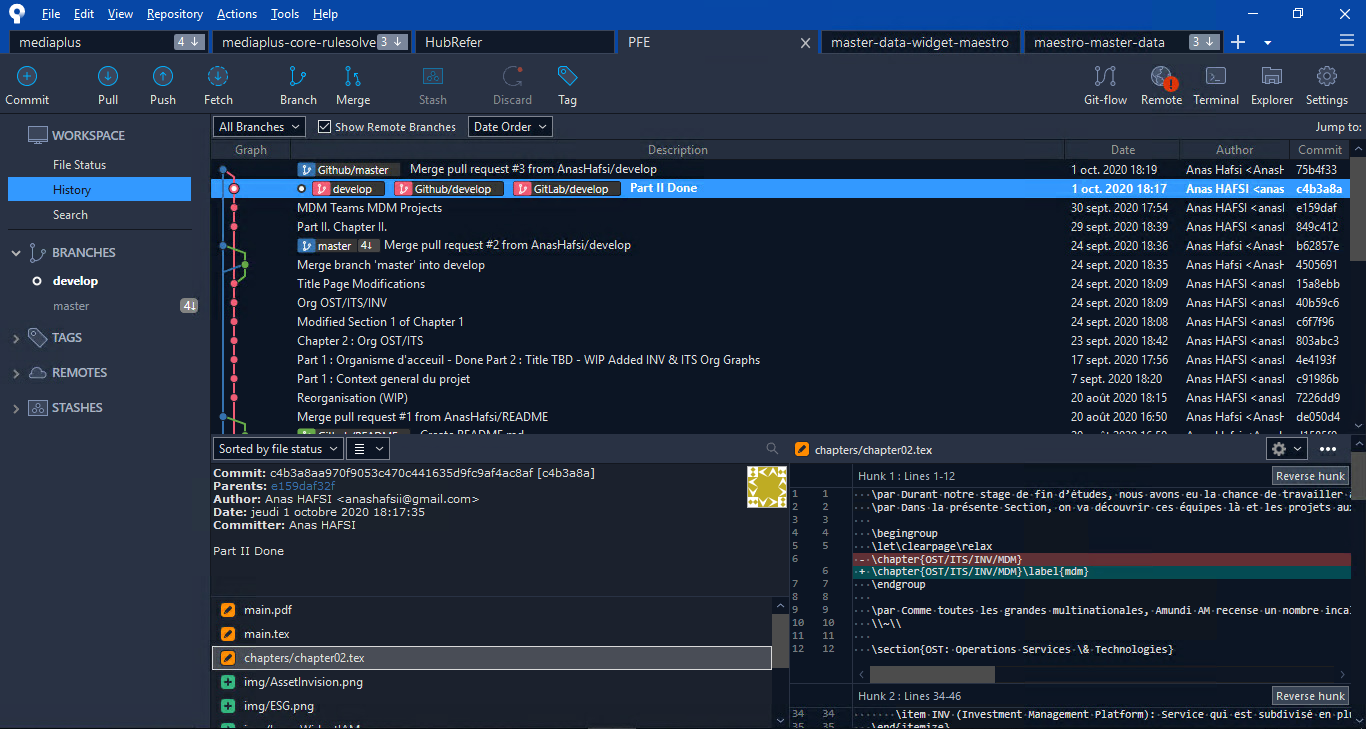
\includegraphics[width=\columnwidth]{img/sourcetree.png}
    \caption{SourceTree: interface pour la branche git contenant mon Rapport de stage}
\end{figure}
\clearpage
\subsection{Jenkins}
\par Jenkins est outil de compilation en continu des sources sur le serveur distant  Git. Il permet le lancement de processus automatiques : Compilation à  récurrence fixe, affichage de la dégradation de la qualité du code, lance les  tests unitaires des projets. Cet outil nécessite énormément de configuration  pour pour commencer à être productif. 
\par Jenkins contient une série de jobs génériques qui ont une utilité particulière. Il  nous est impossible de créer nos propres jobs génériques faute de droits (en  général de besoin. Les jobs génériques couvrent quasiment tous les cas)
\begin{figure}[ht]
    \centering
    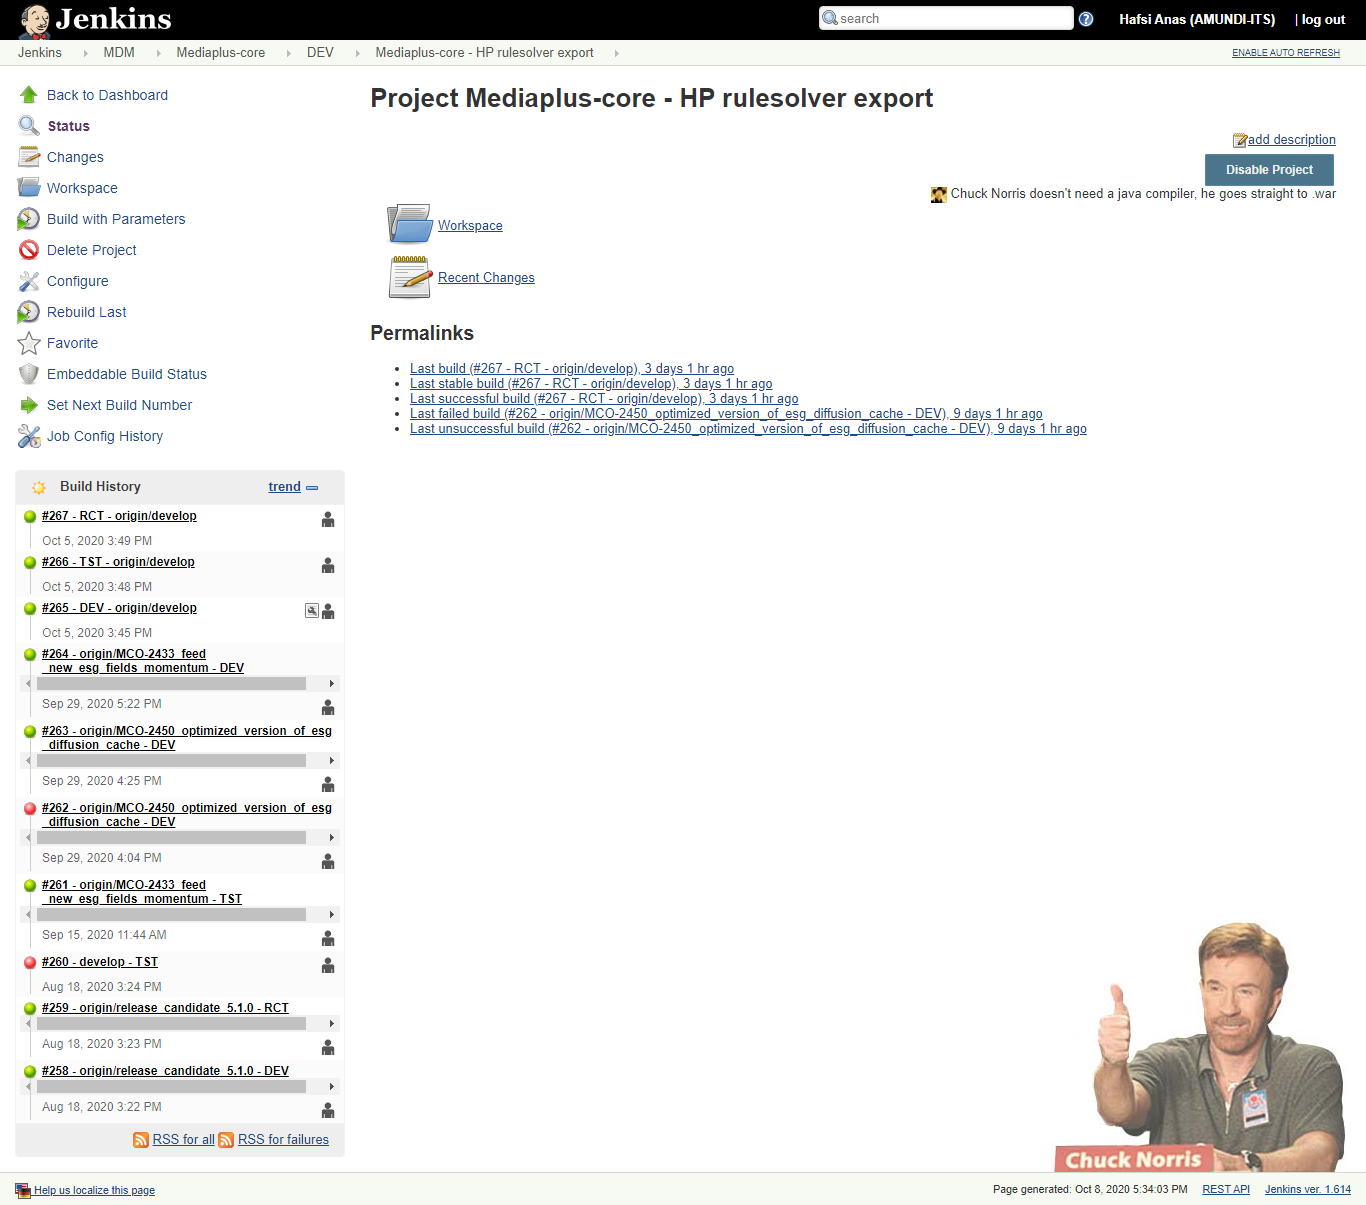
\includegraphics[width=\columnwidth]{img/jenkins.png}
    \caption{Interface Jenkins pour une branche MediaPlus-Core}
\end{figure}
\clearpage
\section{Outils MediaPlus Core}
\par Durant la présente section, on présentera les différents outils technique qu'on a utilisé dans la réalisation des différents tickets JIRA.
\par On va retrouver par exemple des logiciels qui nous permettrons d'accéder au différentes bases de données, des logiciels pour pouvoir faire du monitoring sur l'application MediaPlus-Core des différents environnements (DEV, TEST, RCT, PPR, PROD), pour gérer les differents caches disponibles sur l'application mais aussi pour pouvoir récupérer les différentes données.

\subsection{SQuirreL}
\par SQuirreL SQL Client est une interface graphique open source qui vous permet de visualiser la structure de bases de données conformes JDBC, charger les données dans des tables, ou encore lancer des requêtes SQL.
\par Développé en JAVA, SQuirreL SQL Client est fourni avec une documentation détaillée pour guider au mieux parmi les nombreuses fonctionnalités proposées.
\begin{figure}[ht]
    \centering
    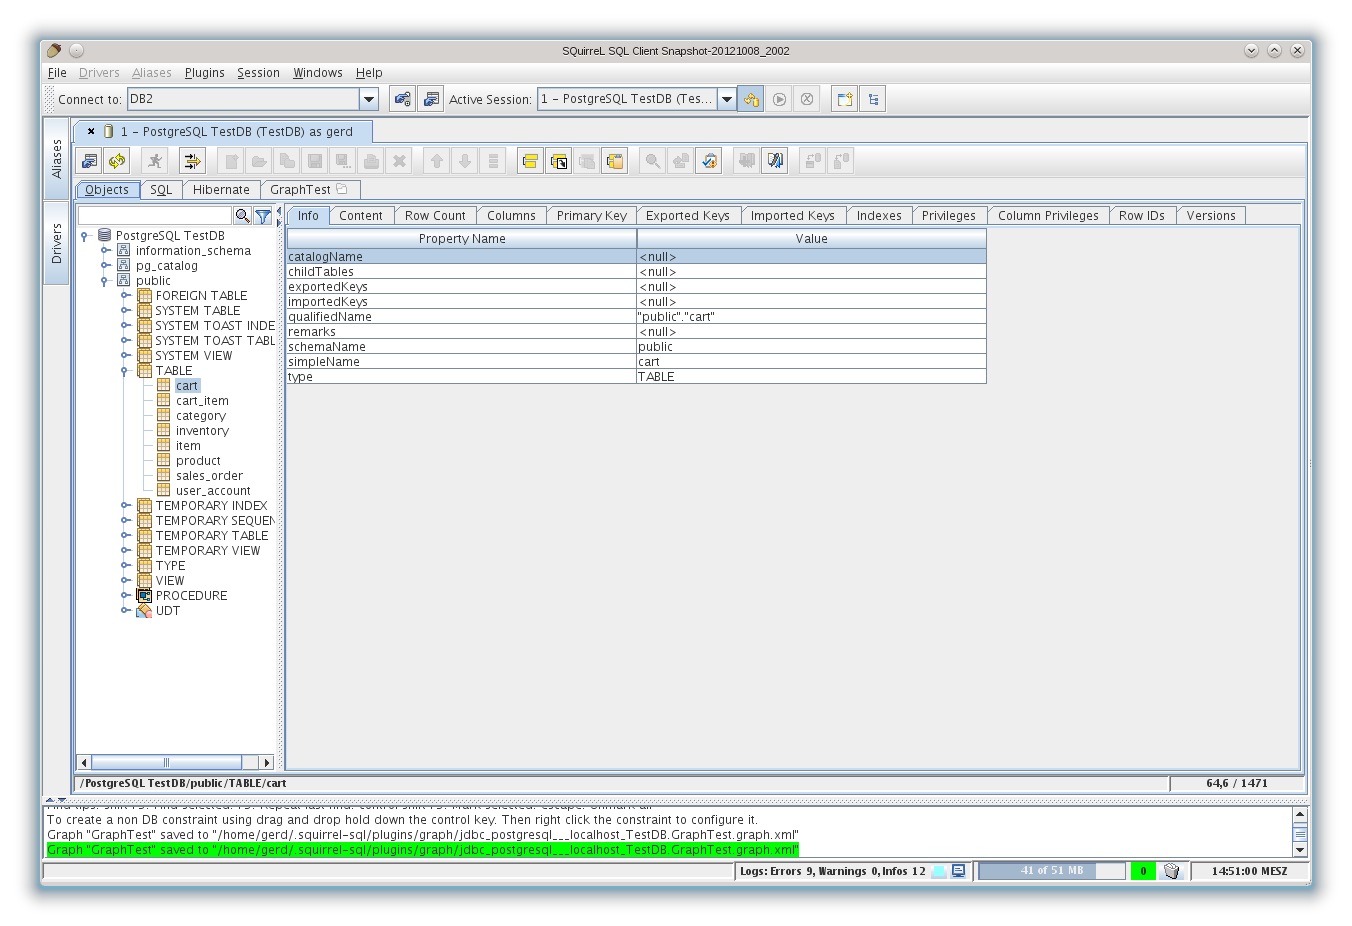
\includegraphics[width=\columnwidth]{img/sqrl.png}
    \caption{Interface SQuirreL}
\end{figure}
\subsection{Server Admin}
\par Comme le nom l'indique, cette application front est considéré comme un administrateur de tout les serveur/applications Amundi-ITS (Exemple: Refgt, Alto, Medco\dots).
\par Cette application, développé pendant les premières années d'activité d'Amundi AM (pour des raisons de confidentialité je ne citerais pas la date), regroupe trois fonctions majeurs, le monitoring, la gestion et l'affichage de donnée.
\begin{itemize}
    \item Monitoring: Permet de surveiller et contrôler le serveur MediaPlus-Core.
    \item Gestion: Permet de contrôler les differents caches MediaPlus-Core (supprimer, recharger, décharger, sérialiser, desérialiser).
    \item Affichage: Afficher les différentes données diffusé par les Ejb MediaPlus-Core.
\end{itemize}
\par La figure \ref{fig:serveradmin} représente l'interface de la partie MediaPlus-core dans ServerAdmin. Des champs ont été caché pour des raisons de confidentialité.
\begin{figure}[ht]
    \centering
    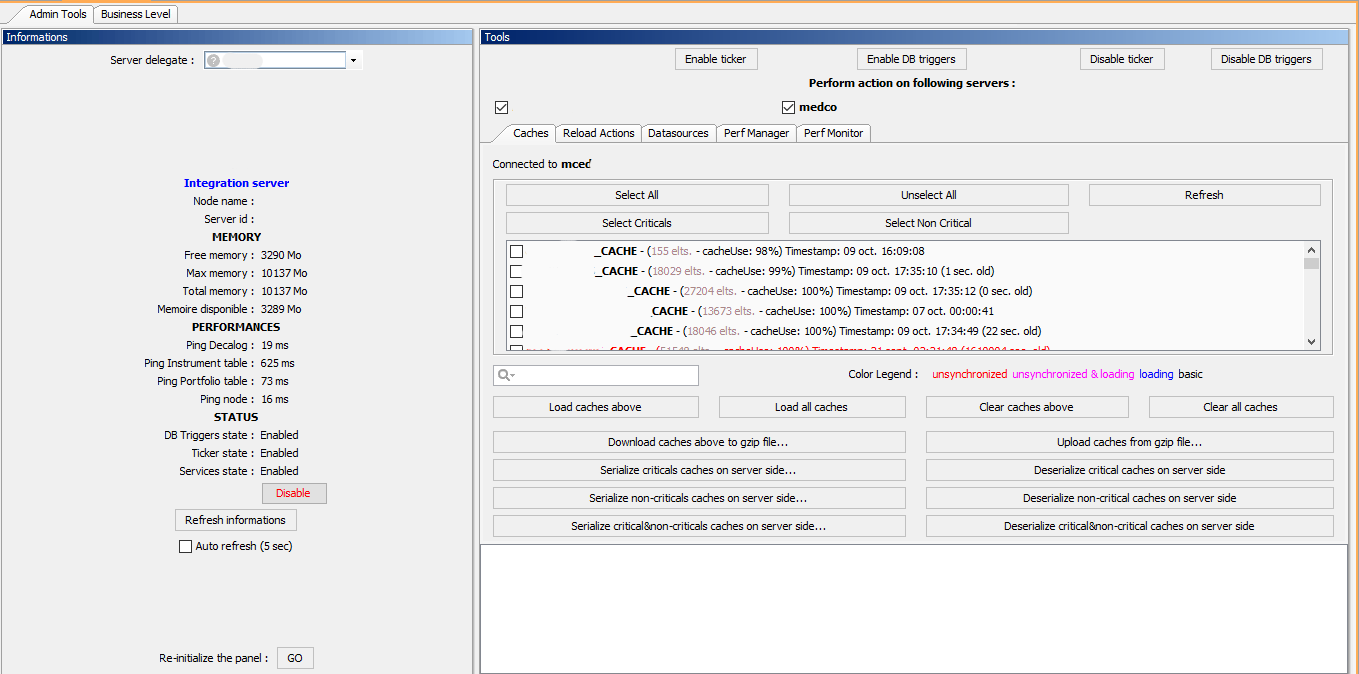
\includegraphics[width=\columnwidth]{img/serveradmin.png}
    \caption{Server Admin}
    \label{fig:serveradmin}
\end{figure}

\subsection{Apache Maven}
\par Apache Maven (couramment appelé Maven) est un outil de gestion et d'automatisation de production des projets logiciels Java en général et Java EE en particulier. Il est utilisé pour automatiser l'intégration continue lors d'un développement de logiciel. Maven est géré par l'organisation Apache Software Foundation. L'outil était précédemment une branche de l'organisation Jakarta Project.
\par L'objectif recherché est de produire un logiciel à partir de ses sources, en optimisant les tâches réalisées à cette fin et en garantissant le bon ordre de fabrication. Il peut se comparer au système make sous Unix ou à l'outil Ant.
\par Maven utilise un paradigme connu sous le nom de Project Object Model (POM) afin de décrire un projet logiciel, ses dépendances avec des modules externes et l'ordre à suivre pour sa production. Il est livré avec un grand nombre de tâches pré-définies, comme la compilation de code Java ou encore sa modularisation.
\par Un élément clé et relativement spécifique de Maven est son aptitude à fonctionner en réseau. Une des motivations historiques de cet outil est de fournir un moyen de synchroniser des projets indépendants : publication standardisée d'information, distribution automatique de modules jar. Ainsi en version de base, Maven peut dynamiquement télécharger du matériel à partir des dépôts logiciels connus. Il propose ainsi la synchronisation transparente de modules nécessaires.
\par L'architecture Maven du projet est disponible dans la figure \ref{fig:mavenarch}. \\
\begin{figure}[ht]
    \begin{lstlisting}
    MediaPlus-Core
    |-- pom.xml
    `-- mediaplus-core-batch
        |-- pom.xml
    `-- mediaplus-core-dist
        |-- pom.xml
    `-- mediaplus-core-ejb
        |-- pom.xml
    `-- mediaplus-core-ejb-server
        |-- pom.xml
    `-- mediaplus-core-server
        |-- pom.xml
    `-- mediaplus-core-to-openaml
        |-- pom.xml
    `-- mediaplus-core-ws
        |-- pom.xml
    `-- mediaplus-core-ws-api
        |-- pom.xml
    `-- mediaplus-core-ws-doc
        |-- pom.xml
    `-- launchers
        `-- local
    `-- doc
    \end{lstlisting}
    \caption{Archetype Maven}
    \label{fig:mavenarch}
\end{figure}
\clearpage
\section{Outils Alto Investment Research}
\par En ce qui concerne Alto Investment Research, on a utilisé, en plus des outils communs, InVision et la documentation Maestro.
\subsection{InVisionApp}
\par InVision est une application accessible par navigateur Internet (SaaS) qui vous permet de présenter vos visuels à même le navigateur du client qui verra exactement de quoi son projet a l’air sur son écran. On évite ainsi toutes les questions et commentaires du type « C’est beau comme ça, mais ça va avoir l’air de quoi dans mon navigateur? » ou encore « Ça a l’air petit dans votre PDF ». Les JPG que vous téléversez dans l’application sont affichés à 100\% de leur dimension et centrés dans l’écran. Il est toutefois possible de jouer avec les paramètres si votre image doit être alignée sur un côté. De plus, InVision met à votre disposition des gabarits de base pour mobile et tablette.
\par Dans la version pro d’InVision (La version Pro utilisé par Amundi AM), il est possible de gérer plusieurs projets en même temps. Chaque projet possède sa propre adresse URL aléatoire. Ainsi, un client ne pourra pas tomber par hasard sur le projet d’un autre client.
\par Les designers de l'équipe "ITS/INV/EAX Entreprise Architecture \& UX Design" réalisent les maquettes (exemple: figure \ref{fig:invision}) sur InVision, et à travers les MOE on récupère les écrans a développer pour réaliser un résultat proche de celui des EAX.
\clearpage
\begin{figure}[ht]
    \centering
    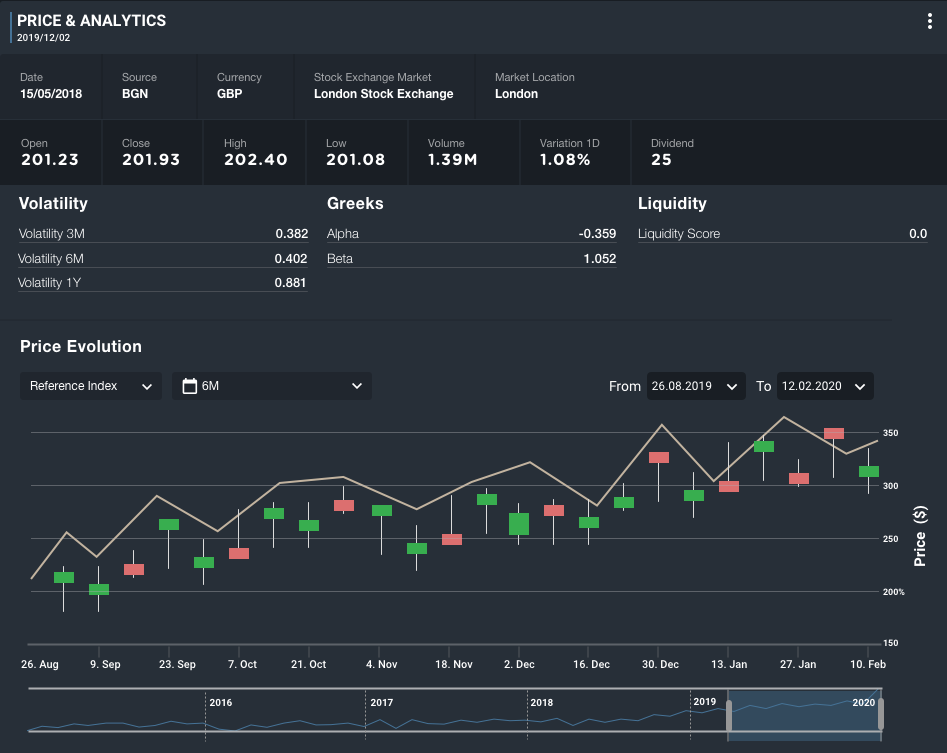
\includegraphics[width=\columnwidth]{img/AssetInvision.png}
    \caption{Exemple d'une maquette ALTO sur InVision}
    \label{fig:invision}
\end{figure} 

\subsection{Documentation Maestro}
\par Comme c'est déjà mentionné dans les chapitres précédents, Maestro est un framework interne Amundi AM basé sur Angular développé par l'équipe ITS/DOT/COR, inclus plusieurs surcouches unifiant toutes les applications front Amundi AM, pouvant parfois faciliter des blocs de code.
\par Pour ce ITS/DOT/COR a mis a notre disposition une documentation complete de tout les composant Maestro ajouté par le framework, ainsi que plusieurs exemples de leurs utilisations.
\begin{figure}[ht]
    \centering
    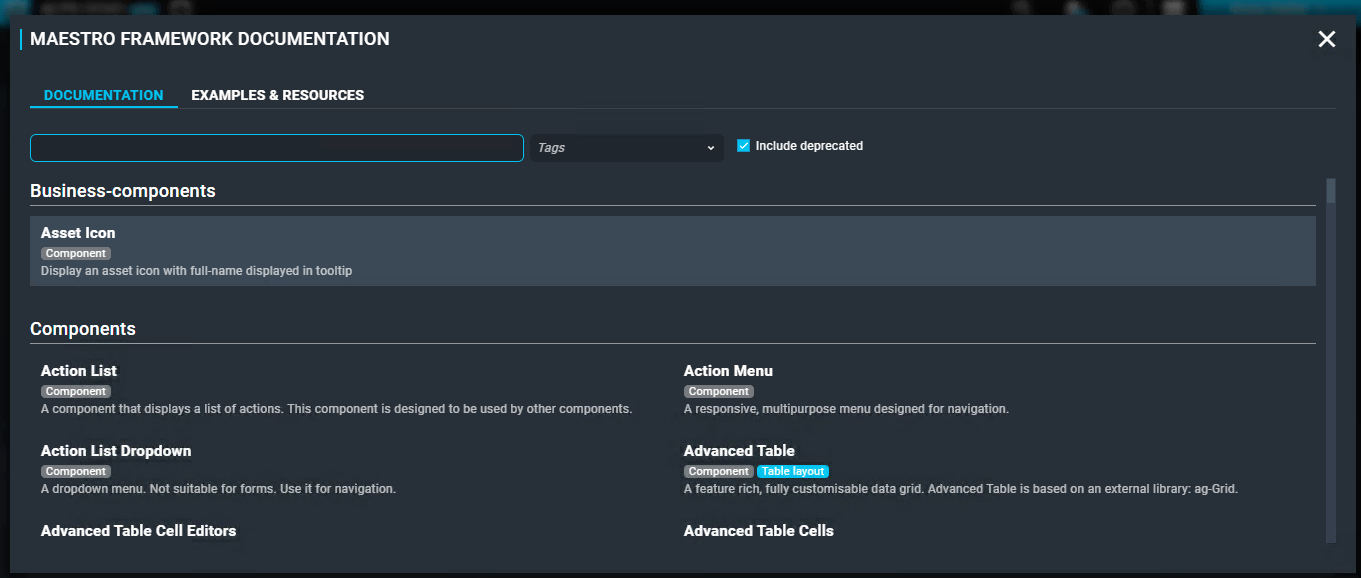
\includegraphics[width=\columnwidth]{img/maestrodocum.png}
    \caption{Exemple de la documentation Maestro}
\end{figure} 

\chapter{Travail réalisé}
\par Dans le présent chapitre on essayera de parler de tout le travail réalisé durant la période passé chez le client ainsi que l'évolution des differents projets auquel j'ai eu la chance de participer.
\section{MediaPlus-Core}
\par Durant mon stage, j'ai eu l'occasion de relisé plusieurs tickets JIRA touchant a plusieurs aspects de l'application MediaPlus-Core. J'ai pu les subdiviser en deux parties: la migration/creation de nouveaux API, et la réalisation de support requests d'autres équipes Amundi AM.
\begin{itemize}
    \item Partie API: J'ai pu créer de nouveaux API et/ou de migrer d'autres depuis le système STPML qui est déprécié au sein d'Amundi vers le system OpenAML.
    \item Support requests: Parfois des ingénieurs Amundi AM (que ça soit des développeurs ou des métiers) ont besoin d'avoir de nouveau champs diffusé par Medco oui remappé vers de nouvelles valeurs depuis les différentes bases de données. 
\end{itemize} 
\par Pour des raisons de confidentialité, je me passerais de plusieurs details (notamment noms (deuxième API) et details techniques).
\subsection{Creation d'API REST}
\par Après avoir rejoint l'équipe Medco, J'ai pu développer (from scratch) deux nouvelles API.\\
\begin{itemize}
    \item Countries: L'API des countries est un API essentiel pour le fonctionnement d'autres API ainsi que la diffusions de plusieurs champs. En effet on peut le retrouver dans plusieurs types de données (Exemple: Currency/Devise qui est un Objet indispensable dans le domaine financier). L'API était précédemment diffusé sous format STPML, format déclaré obsolète, et donc fallait migrer et remapper les objets pour pouvoir être compatible. L'API, accessible ar l'URL medco/countries, dispose d'une fonctionnalité de recherche par identifiant, un identifiant obéissant au format ISO 3166-1 alpha-3, accessible par l'URL medco/country/ISO. L'API était doté d'un mécanisme de filtrage/recherche plus puissant qui permettait de filter tout les country par champs, le critère de filtrage était passé par url params. Par exemple je pouvait chercher tout les pays avec un iso débutant par "A" j'utilisait l'URL medco/country?ISO=A.* ou si je voulais diffuser les pays membre de la zone euro j'utilise medco/country?euroZone=true. Pour des raisons de confidentialité, le nombre de champs diffusé reste inconnu mais le mécanisme de recherche était fonctionnel pour un très grand nombre de champs (plus de 10). \\
    \item L'API qu'on nommera Entity: cet objet est un objet sensible au sein de l'écosystème Amundi AM, du coup plusieurs details seront caché. Comme pour les countries, Entity est une données très importante pour les ingénieurs Amundi AM, Seule différence est que l'API n'existait pas sous le format STPML (en tout cas pas dans le format actuel de la data), du coup il fallait coder le mapping OpenAML. En plus des caractéristique précédemment cité dans la partie API Country (recherche par champs\dots), cet API dispose d'un autre paramètres de filtrage qui nous permet d'afficher ou non des champs de data en fonction de l'Entity utilisé, on peut diffuser jusqu'à trois niveaux de data, le niveau le plus bas étant le moins complexe. \\
\end{itemize}
\subsection{Support Request}
\par Comme c'est déjà mentionné, la partie support request concernait la partie interaction avec les differents utilisateurs Amundi AM. 
\par L'équipes recevait plusieurs demandes dont on peut citer: \\
\begin{itemize}
    \item Ajout de champs: Support request le plus reçu par l'équipe. Si une équipe a besoin de diffuser un nouveau champs depuis le différentes bases de données, l'équipe Medco récupère la demande sous forme de ticket JIRA et essaye de la traiter en modifiant les ejb pour diffuser le nouveau champs.
    \item Remapping de champs: Au cas ou une équipe essaye de changer le mapping pré-crée, l'équipe se charge, après avoir reçu l'accord des équipe métier concerné par le champ, de le faire tout en alertant les autres équipes gérant des projets ou le champ était utilisé. 
    \item Suppression de champs: La suppression de champ est une operation rare dans l'équipe Medco. Elle occurre généralement lorsqu'un champ est obsolète ou dont la diffusion peut engendrer des erreurs dans les résultats émis par d'autres champs/services. Comme pour le remapping, l'équipe contacte les gestionnaire métier du champs, pour avoir une confirmation et procède à la suppression de champs tout en notifiant les équipes pouvant utiliser le champ en question.
\end{itemize}
\par De mon coté j'ai pu traiter les deux premiers types de support requests à savoir la creation et le remapping de champs. 
\section{Alto Investment Research}
\par Sur Alto Investment Research Referential Widgets, le but était de reproduire les designs présent sur InVision par ordre proposé par Sara Hilmi MOA Front Office, de l'équipe GES/COO/GIS/MFO.
\par Avant ma venue dans l'équipe, les widgets présents sur Alto Investment Research était sous le format présent dans la figure \ref{fig:altoV1}.
\begin{figure}[ht]
    \centering
    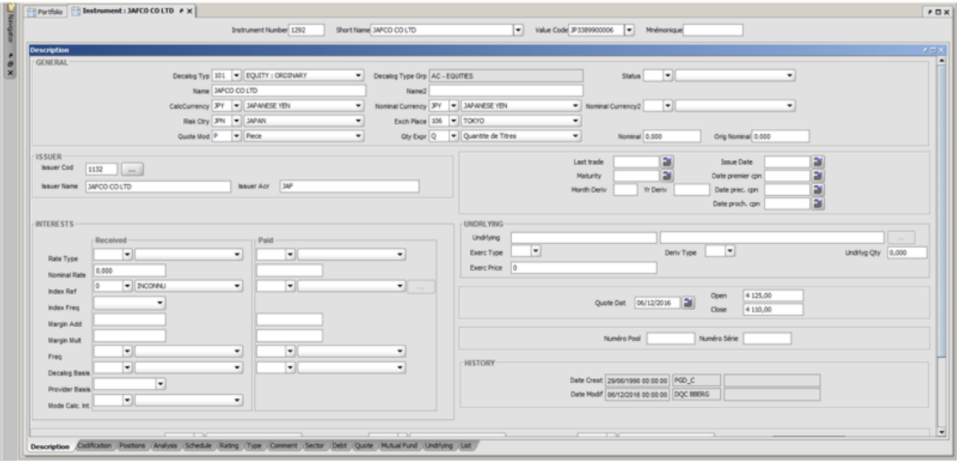
\includegraphics[width=\columnwidth]{img/ancienecrans.png}
    \caption{Anciens Écrans d'Alto Investment Research}
    \label{fig:altoV1}
\end{figure} 
\par Le but était de répliquer les écrans figurant dans la figure \ref{fig:altoInv}.
\par Le résultat réalisé figure dans la figure \ref{fig:altoCurent}.
\par Plusieurs informations ont ete modifiée pour des raisons de confidentialité.
\par Mon travail consistait a réaliser les écrans (partie front), ainsi que les API Maestro pour récupérer la data depuis les differents serveurs et applications Medco (Refgt et Hubref).
\begin{figure}[ht]
    \centering
    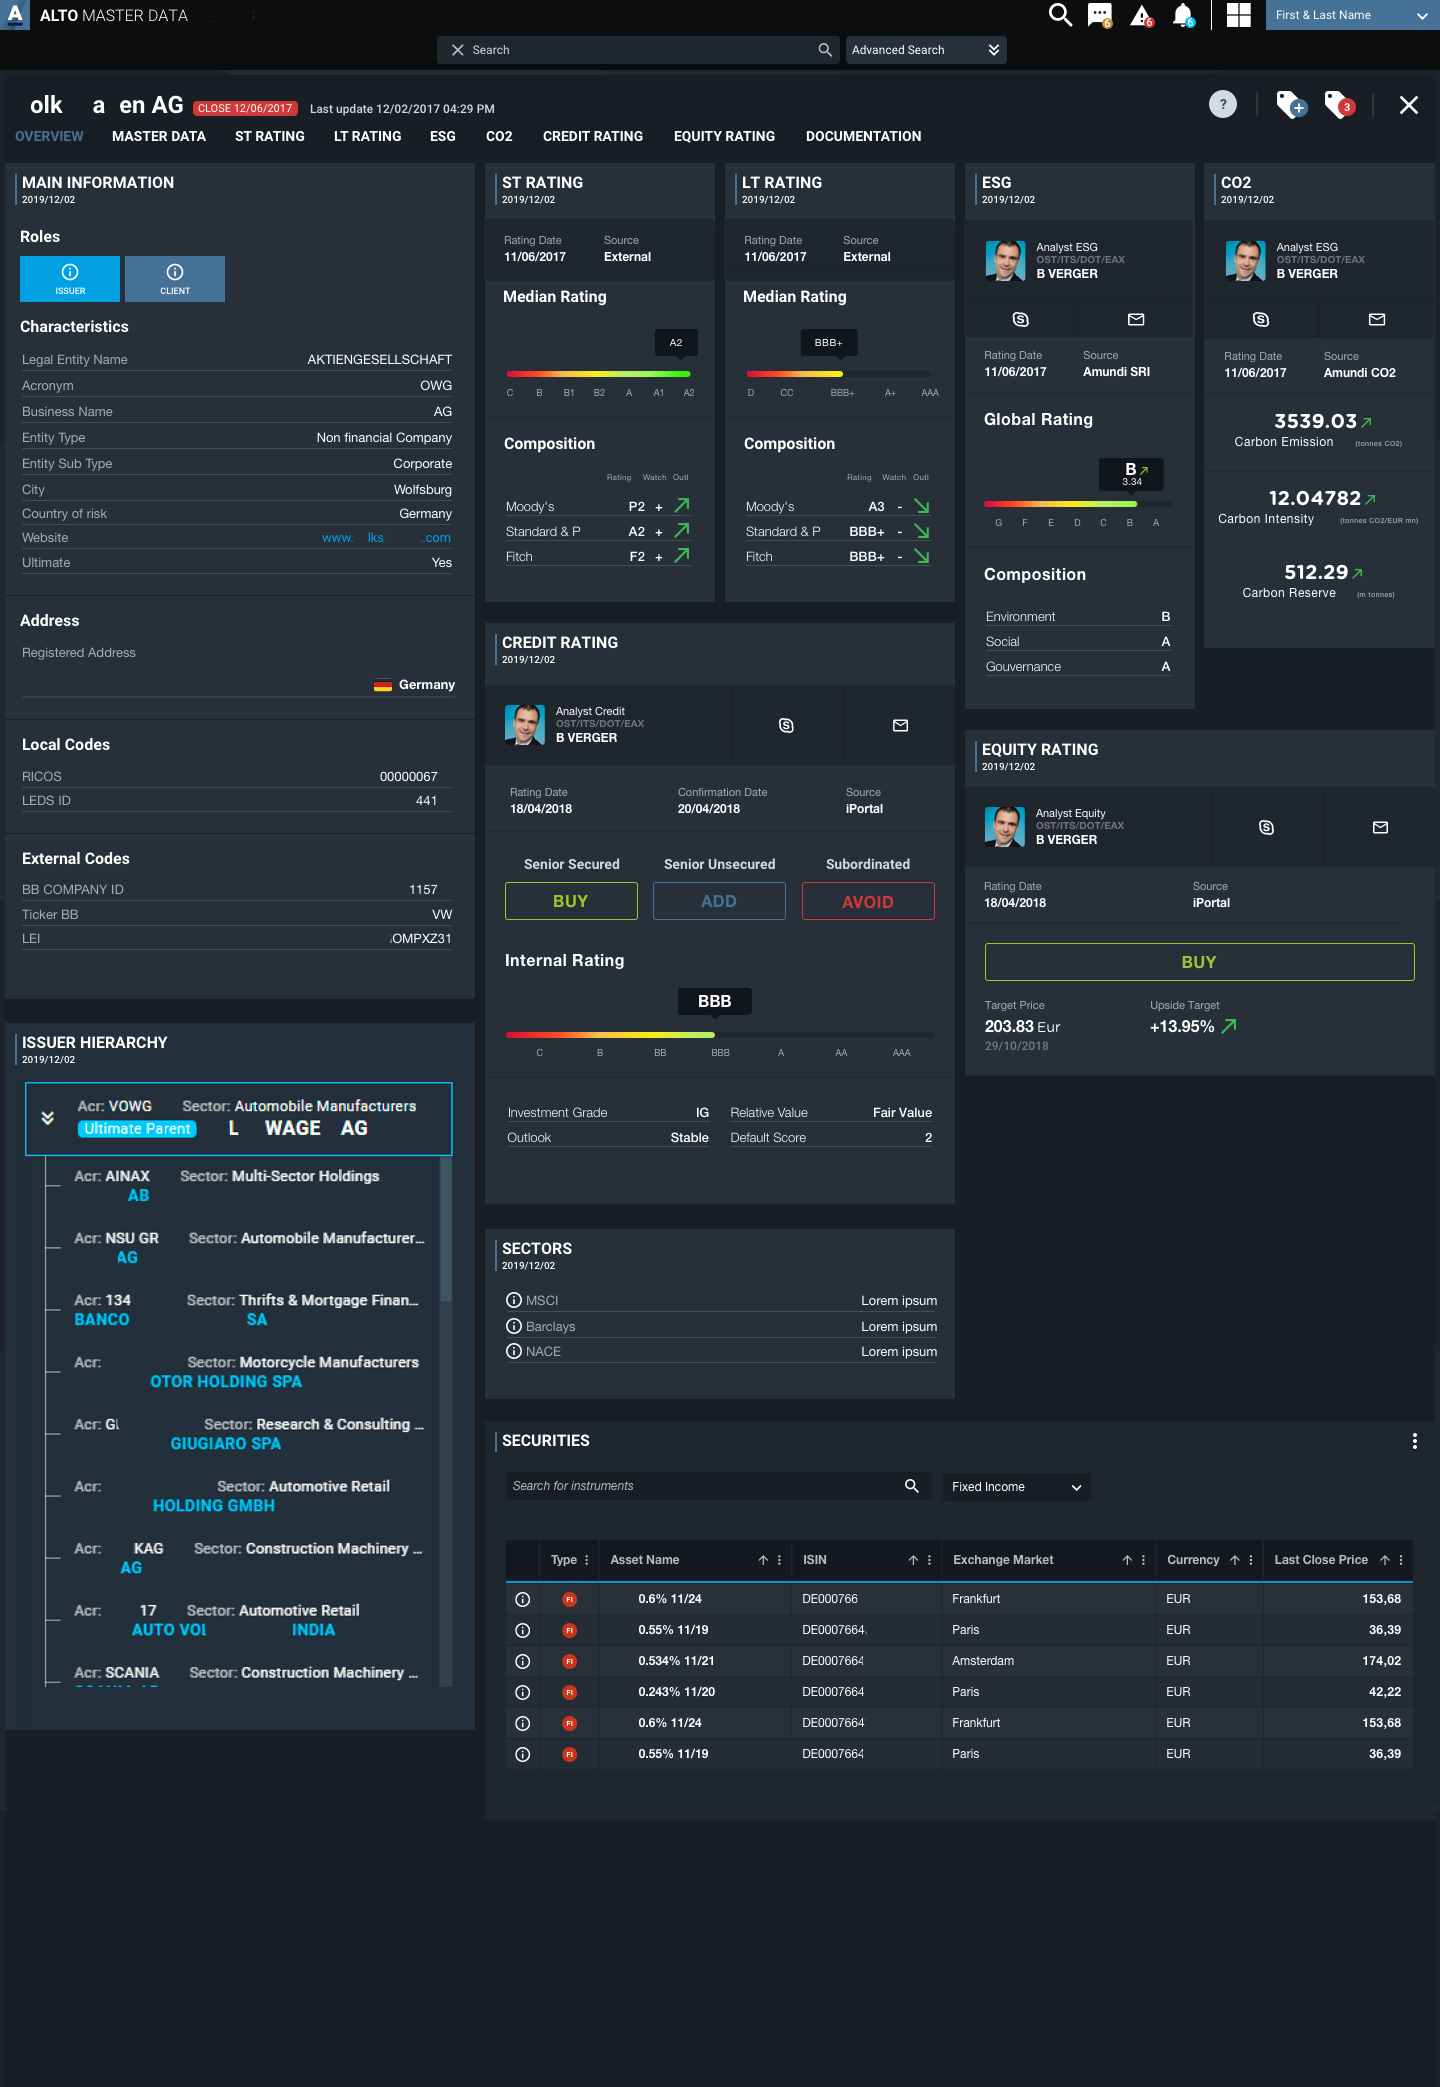
\includegraphics[width=\columnwidth]{img/invisionEx.png}
    \caption{Résultat attendu depuis Invision}
    \label{fig:altoInv}
\end{figure}
\begin{figure}[ht]
    \centering
    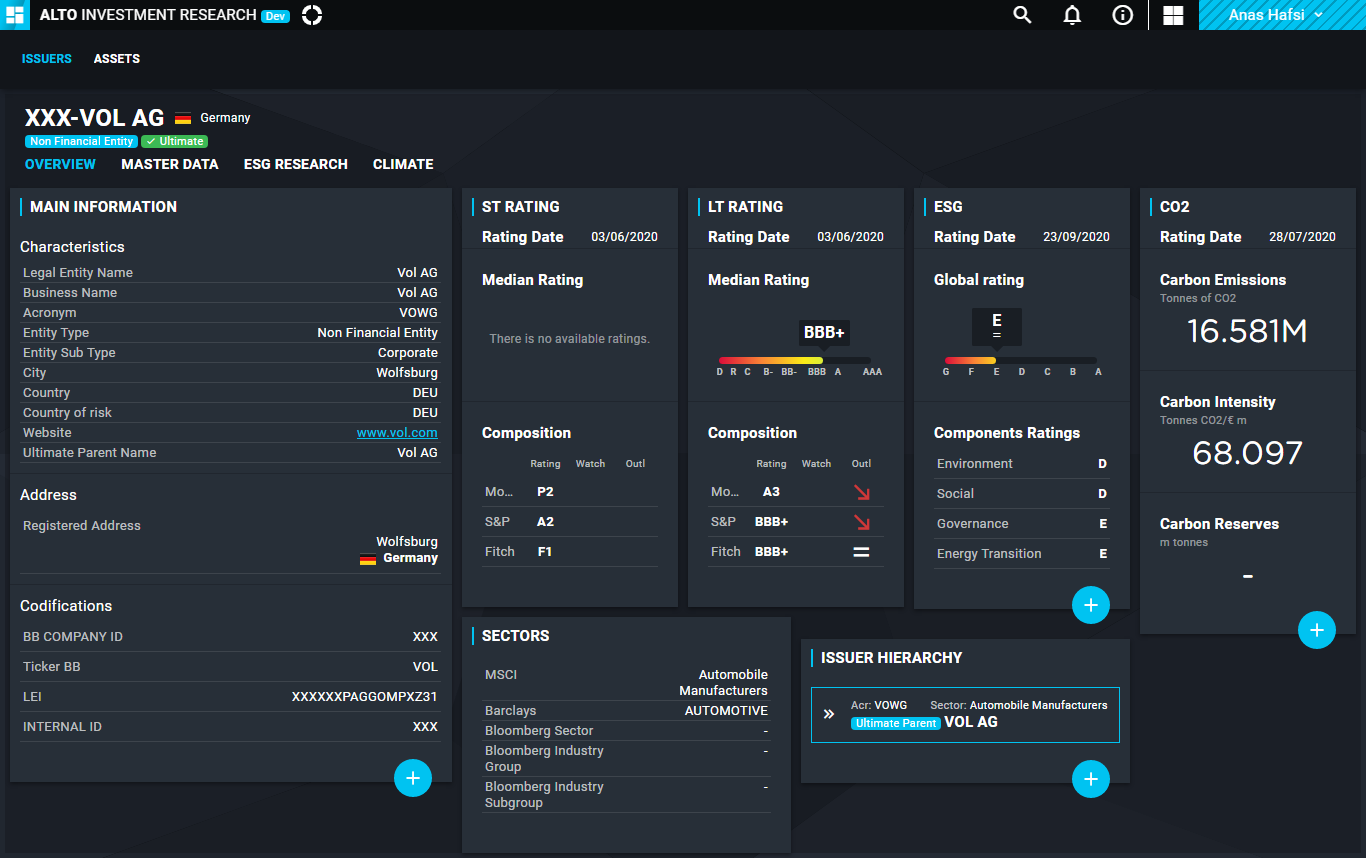
\includegraphics[width=\columnwidth]{img/investmentRsch.png}
    \caption{Version actuelle d'Alto Investment Research}
    \label{fig:altoCurent}
\end{figure}
\chapter{Conclusion générale}
\par C'est la conclusion

\end{document}
